% article example for classicthesis.sty
\documentclass[10pt,a4paper]{article} % KOMA-Script article scrartcl
\usepackage{lipsum}
\usepackage{url}
\usepackage[nochapters]{../classicthesis} % nochapters
\usepackage{graphicx}
\usepackage{booktabs}
\usepackage{float}


\begin{document}
    \pagestyle{plain}
    \title{\rmfamily\normalfont\spacedallcaps{Mission: Chuckhole}}
    \author{\spacedlowsmallcaps{Marwan ElMezni, Michael Moosbauer}}
    \date{} % no date
    
    \maketitle
    
%    \begin{abstract}
        %Maybe we won't need an abstract
 %   \end{abstract}
       
    \tableofcontents
    
    \section{Ideation}
\subsection  {Problem statement}
\begin{itemize}
\item \textit{What is the context of the problem? }

Many roads are damaged because of different causes.
\item \textit{Why is it a problem?}

Bad quality of roads damages vehicles and may interrupt or slow the traffic.
\item \textit{Who has the problem?}

Bike riders or vehicles owners.
Municipalities trying to maintain roads in a good quality.


\end{itemize}

     	

\subsection{Steps to Personas / Personas}
\begin{itemize}
\item Finding users

\begin{itemize}
\item \textit{Who are they?}

Bike riders, vehicles owners and municipalities trying to maintain roads in a good quality.

\item \textit{How many are they?}

Theoretically, the app would attract a lot of users.

\item  	\textit{What do they do with the system?}

\begin{itemize}
\item Check instantly the quality of roads while riding their bikes.

\item Detect and localize chuckholes thanks to heatmaps and markers on the map.

\item Avoid riding on damaged roads thanks to heatmaps.
\end{itemize}

\end{itemize}

 \end{itemize}   
 
 \begin{itemize}
\item Building a hypothesis
 \begin{itemize}
 \item  	\textit{What are the differences between the users?}
 
 Some users want just to avoid chuckholes during their bike rides while others will have fun to utilize the app or need it for specific reasons. 
 \end{itemize}
  \end{itemize}
   
   \begin{itemize}
\item Verification

Personas: Municipalities’ agents and bikers.
 
   \end{itemize} 
 
 
   
   \begin{itemize}
   
\item Finding patterns
 \begin{itemize}
 \item  	 	\textit{Does the initial grouping hold? Are there other groups to consider?}
\begin{itemize}
 \item  The initial grouping done in the previous step still holds.
 \item No more groups to consider by now.
\end{itemize} 
 \item  	\textit{Are all equally important?}
 
 Municipalities’ agents and some groups of bikers may have more importance:  more active users that will frequently use the app and evaluate its functionalities much deeper than others who would be contented to use specific features.
 
   \end{itemize} 
   
   
  \item Constructing personas
   
   
   \begin{table}[ht]
\centering
\label{my-label}
\resizebox{\textwidth}{!}{%
\begin{tabular}{@{}c|c|c|c|@{}}
\cmidrule(l){2-4}
                                                          & \textbf{Martin}                                                                                                                                                                                                               & \textbf{Anna}        & \textbf{Andreas}                                                                                                             \\ \midrule
\multicolumn{1}{|c|}{Character}                           & Extrovert                                                                                                                                                                                                                     & Extrovert            & Introvert                                                                                                                    \\ \midrule
\multicolumn{1}{|c|}{Age}                                 & 30 yo                                                                                                                                                                                                                         & 22 yo                & 45 yo                                                                                                                        \\ \midrule
\multicolumn{1}{|c|}{Occupation}                          & Officer and professional biker                                                                                                                                                                                                & Student              & Municipality's agent                                                                                                         \\ \midrule
\multicolumn{1}{|c|}{Interest}                            & \begin{tabular}[c]{@{}c@{}}High interest in the\\ app and uses frequently all features.\end{tabular}                                                                                                                          & Normal interest      & Interest due to his work duties                                                                                              \\ \midrule
\multicolumn{1}{|c|}{When does the user utilize the app?} & Weekends                                                                                                                                                                                                                      & No particular time   & Weekdays                                                                                                                     \\ \midrule
\multicolumn{1}{|c|}{Why?}                                & \multicolumn{1}{l|}{\begin{tabular}[c]{@{}l@{}}- Detect and localize chuckholes.\\ - Avoid chuckholes\\ and ride across smooth sections.\\ - Test the app performance and suggest\\ improvements or extensions.\end{tabular}} & Avoid chuckholes and & \begin{tabular}[c]{@{}c@{}}Use the app to detect\\ new chuckholes or to \\ localize old chuckholes to be fixed.\end{tabular} \\ \bottomrule
\end{tabular}%
}
\end{table}



\item Defining situations

\begin{itemize}
 \item  	\textit{What are the needs of this persona?}
 \item  	\textit{What are the situations?}


 \end{itemize} 
 
 
 \item Validation

 \end{itemize} 
 
 
 
 
 
\subsection  {Scenarios}
 
 
 
 
 
 
    \section{Recommended Setup}
	%photo of bike, smartphone fix, ...    
	\begin{itemize} 
	\item Bike: Drössiger 650B full suspension.
	\item Smartphone (Samsung Galaxy S4 Active).
	\item Fix spot of the mobile phone: ???
	
	
	\end{itemize}
	% send me a picture of your bike with the fix and the phone
	
	


    \section{Architecture}
	% maybe UML class diagram, if suitable
	
	\begin{figure}[H]
	\centering
    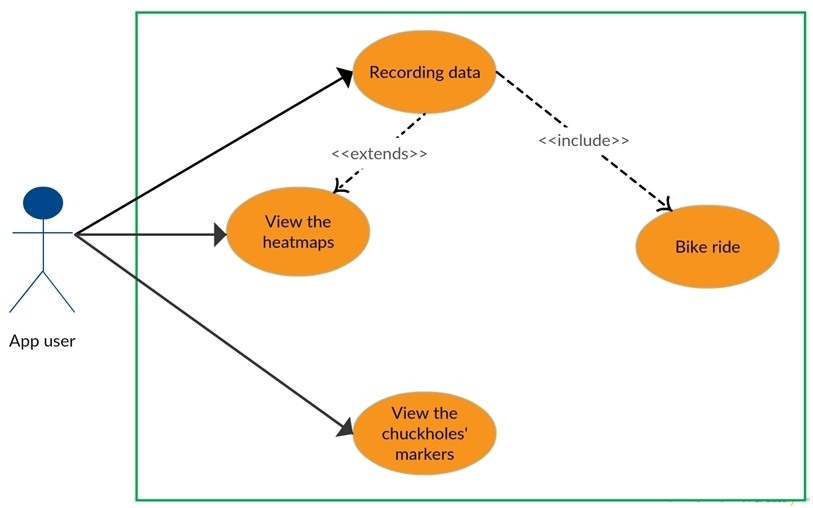
\includegraphics[width=16cm, height=12cm]{UML}
    
    \end{figure}
    
    \section{App Features}
	% pictures etc. here
    
    
    % bib stuff
    \nocite{*}
    \addtocontents{toc}{\protect\vspace{\beforebibskip}}
    \addcontentsline{toc}{section}{\refname}    
    \bibliographystyle{plain}
    \bibliography{../Bibliography}
\end{document}
